\documentclass{article}
\usepackage{geometry}
\geometry{letterpaper, margin=0.85in}
\usepackage{amsmath}
\usepackage{graphicx}
\usepackage{amssymb}
\usepackage[utf8]{inputenc}
\title{Beaver Works Summer Institute 2018\\Unmanned Aerial Vehicle}
\author{Spencer Ng}
\date{}
\begin{document}
\maketitle
\section*{Drone Architecture}
\begin{itemize}
\item Two main control systems
		\item  AeroFC responsible for just flight, very low level (PX4)
		\item  Aero Compute Board is high level, using ROS as middleware

\end{itemize}

\section*{Robotics Operating System (ROS)}
\begin{itemize}
\item Use \verb|rostopic echo <topic>| to print from a topic
\item MAVROS is for AeroFC, ROS is for Aero Compute Controller
\item Nodes subscribe and publish to topics\begin{itemize}
\item Make decisions based on messages sent by other nodes
\end{itemize}
\end{itemize}
\section*{Localization Techniques}
\begin{itemize}
\item Need to recognize where the drone is in the room or relative to frame of reference (origin)
\item  Includes velocity, pitch, roll
\item Techniques include
\begin{itemize}
\item Dead reckoning
\begin{itemize}
\item Using gyros, accelerometers, pots to determine how much a plant has moved
\item Not good due to external inputs (e.g. wind)
\end{itemize}
\item GPS
\begin{itemize}
\item Gives a very good signal
\item Precision only within meters
\item Can't use indoors
\end{itemize}
\item Radio Frequency/Ultra Wideband
\begin{itemize}
\item Good for controlled environments, needs to be set up
\end{itemize}
\item Motion capture
\begin{itemize}
\item Fast and reliable
\item Very popular for research due to high precision
\item Only good for dedicated rooms and expensive
\item Unrealistic
\end{itemize}
\item Visual Odometry
\begin{itemize}
\item How we navigate, with a visual map
\end{itemize}
\item SLAM (Simultaneous Localization And Mapping)
\begin{itemize}
\item Creates a map and tries to localize at the same time
\item Huge issue in robotics today, in terms of accuracy and performance
\item IntelAero is capable, but is difficult to achieve well
\item  Active area of research
\end{itemize}
\end{itemize}
\end{itemize}
\section*{Reference Frames}
\begin{itemize}
\item Need to understand quadrotor reference frame with respect to the world
\item Either inertial or non-inertial (not accelerating, may be at constant nonzero velocity)
\item NED or ENU is the world reference frame
\begin{itemize}
\item $+z$ is down in NED (north east down)
\item $+z$ is up in ENU (east north up)
\item $+x$ is north and $+y$ is east in NED,  vice versa in ENU
\end{itemize}
\item Body frame (quadrotor)
\begin{itemize}
\item $+x$ toward front
\item $+z$ down
\item $+y$ toward right "wing"
\item Origin is at center of mass
\end{itemize}
\item Marker frame is attached to AR marker
\begin{itemize}
\item Why tags are so useful
\end{itemize}
\item Transformations can be made mathematically
\end{itemize}
\section*{Convolutions}
\begin{itemize}
	\item Moving average of intensity values in a grid produces edges 
      \begin{itemize}
      \item Smoothing function to suppress noise but makes it blurrier 
      \end{itemize}
	\item Image segmentation based on threshold 
      \begin{itemize}
      \item If above, make white; otherwise, change to black 
      \end{itemize}
    \item Shift invariance 
    \item Linear filters 
    \item To handle boundaries, duplicating parts of the image rather than leaving an edge produces a better result after running blurring kernel 
    \item Kernels are matrices for filters 
      \begin{itemize}
      \item Sobels are for edge detection, starting from a particular direction 
      \item New pixel intensity is equal to "cross product" of kernel with adjacent pixels, equal to kernel size 
      \end{itemize}
	\item Linear regression - extract lines out of an image 
      \begin{itemize}
      \item Algebraic approach involves computing averages of the points to minimize squared error
      \item Machine learning: guess and check from points (RANSAC technique)
      \begin{itemize}
      \item Two parameters: slope and intercept 
      \item Draw a line through two points at random, set "thresholds," determine how many "inliers" and outliers 
      \begin{itemize}
      \item Measure distance from every point to that line (either vertical/least squares or normal)
      \item Distance is the cost to minimize
      \end{itemize}
      \item Rinse and repeat until inliers increase in number, until there's a good line 
      \item "Hopping around" the slope vs intercept vs squared error graph, for a set number of iterations 
      \item Convex optimization – not all problems have a definite curve to minimize error 
      \begin{itemize}
      \item Hard to change parameters and descend "cost hill" 
      \end{itemize}
      \end{itemize}
\end{itemize}
\item Operations
\begin{itemize}
\item Adding
\item Blending
\item Erosion
\item Dilation
\item Rotation
\end{itemize}
\end{itemize}
\section*{Computer Vision}
\begin{itemize}
\item AR tags in use 
\item A .bag file stores raw sensor data 
\item More than light and scene properties? 
\begin{itemize}
\item Optical illusions and human perception is important 
\end{itemize}
\item Edge detection 
\begin{itemize}
\item Use intensity rather than color differences 
\item Makes us capable of recognizing objects 
\item Horizon and vanishing points used for depth perception 
\item Surface discontinuity – based on light, depth, or shadows 
\end{itemize}
\item Computers better than humans at parallel procssing 
\item Goal of vision is to turn binary data into something recognizable 
\begin{itemize}
\item Many applications 
\end{itemize}
\item 3D graph of intensity as a grid of pixels 
\item Image is still a discrete signal, rather than countinuous 
\item Intensity ranges from 0 to 255 
\item Color models are RGB, lab, or HSV 
\item An image can be a function from $\mathbb{R}^2$ to $\mathbb{R}^M$, where $M$ is the number of colors
\begin{itemize}
\item A position $(x,y)$ is converted into $(R,G,B)$
\end{itemize}
\item Images formed either perspective projection (has diagonals) or orthographic projection (only parallel lines) 
\begin{itemize}
\item Orthographic taken from very far away, then zooming in
\end{itemize}
\item Image formation model for three dimensional world 
\begin{itemize}
\item Y and Z axes are meshed togeteher in 2D representation 
\item X is preserved, in the same orientation 
\end{itemize}
\item Edge classification 
\begin{itemize}
\item Figure segmentation 
\item Occlusion edges 
\begin{itemize}
\item Only the foreground 
\end{itemize}
\item Contact edges – touching the ground 
\begin{itemize}
\item Y is 0 because the object is touching the ground 
\item Z value is still unknown 
\end{itemize}
\end{itemize}
\item Accidental image – distorts perception of axes, loses info 
\item Differential geometry - using $(N-1)$-D images to visualize $N$-D objects
\item Systems and filters
\begin{itemize}
\item Goal is to extract feature (edges, blobs) from images 
\item Denoising, in-painting, etc 
\item Linear filter in 1D 
\begin{itemize}
\item A set of $n$ values in an array $g$ 
\item Another signal (sort of like modulating in AM) is introduced to filter/transform that signal 
\item Used to create an overall transformative function,$ f(n) =H(g(n), s(x,y))$
\end{itemize}
\item Translation invariant filter – do same operation at every point in the image to filter it 
\begin{itemize}
\item If input image is filtered by m samples, output also translated by m samples 
\end{itemize}
\item Convolution 
\begin{itemize}
\item Key operation for machine learning/embedded (local) vision 
\item Sliding/multiplying a set of values across another set of values to produce a transformation 
\item Same as cross correlation 
\end{itemize}
\end{itemize}
\item Characterizing edges – place of rapid change in image intensity 
\begin{itemize}
\item First derivative of intensity vs. Position graph (aka gradient profile)  shows spikes/peaks  
\item Noise causes derivative/gradient profile to be unreadable, as there are many edges 
\item Finite differences is susceptible to noise 
\item Smooth/filter by combining the input signal and a bell curve (Gaussian distribution) $f(x)=s(b(x))$ 
\item To detect change in intensity, just take the derivative and use convolution after smoothing 
\item Power rule: $\frac{d}{dx}x^n=n\cdot x^{n-1}$ 
\end{itemize}
\item Deep learning
\begin{itemize}
\item Convolution Neural Networks (CNN) - collections of basic mathematical operations 
\item Training begins with discriminator and generator, which learn from each other 
\item Called "deep" because transformations keep on going further down
\end{itemize}
\item Recurrent Neural Network (RNN)
\begin{itemize}
\item Keep on transforming the image; feed output back into input
\end{itemize}
\end{itemize}
\section*{Color Segmentation}
\begin{itemize}
\item RGB color space – visualized as 3D graph, values 0-255 for each channel 
\item HSL/HSV - polar coordinates, visualized as cylinder
\begin{itemize}
\item Saturation is radius 
\item Lightness/value is height 
\item Hue is degree/direction 
\end{itemize}
\item  Color thresholding – cutoff at particular value 
\item Color masking 
\end{itemize}
\section*{States}
\begin{itemize}
\item State vector contains 12 variables for complete and unique description of quadrotor
    \begin{itemize}
    \item $\dot{\vec{\zeta}}=f(\vec{\zeta},\vec{u})$
      \item $x, y, z$ for position (could be very noisy)
      \item $v_x, v_y, v_z$ for velocity (often calculated or estimated)
      \item $\phi, \theta, \psi$ for roll, pitch, and yaw
      \item $p, q, r$ for pitch, roll, and yaw "velocities"
    \end{itemize}
\end{itemize}

\begin{equation*}
\vec{\zeta}=
\begin{bmatrix}
x\\y\\z\\v_x\\v_y\\v_z\\\phi\\\theta\\\psi\\p\\q\\r
\end{bmatrix}
\end{equation*}

\begin{itemize}
\item $\vec{u}$ contains angular velocities for four rotors $(\omega_1, \omega_2, \omega_3, \omega_4)$
    \begin{itemize}
    \item Derive acceleration/force using $F=m\cdot\vec{a}$ and $\tau=I\cdot\dot{\omega}$
    
    \end{itemize}
   \end{itemize}
   
  \begin{equation*}
    \vec{u}=
    \begin{bmatrix}
    \omega_1\\\omega_2\\\omega_3\\\omega_4
    \end{bmatrix}\rightarrow
    \begin{bmatrix}
    \omega_1^2\\\omega_2^2\\\omega_3^2\\\omega_4^2
    \end{bmatrix}\rightarrow
    \begin{bmatrix}
    f\\\tau_1\\\tau_2\\\tau_3
    \end{bmatrix}
    \end{equation*}
    \begin{itemize}
    \item Above is the low level control, where $f$ is the sum of all forces on four rotors, $\tau_n$ is the torque on the center of mass on the quadrotor, in all three directions
    \item Rightmost vector is what's really used
    \item Physics is mostly handled by the flight controller, which we just send velocity commands to via MAVROS
    \end{itemize}
\begin{equation*}
\begin{split}
\dot{\vec{x}}&=\frac{d^w\vec{x}_B}{dt}\\
\ddot{x}&=mg\vec{z}_w-u_1\vec{z}_b\\
\dot{R}_{BW}&=R_{BW}\vec{\Omega}_{BW}\\
\dot{\vec{\Omega}}_{BW}&=\begin{bmatrix}
u_2\\u_3\\u_4
\end{bmatrix}-\vec{\Omega}_{BW}xJ_B\vec{\Omega}_{BW}
\end{split}
\end{equation*}

\section*{Controls \& Estimation}
\begin{itemize}
\item Three aspects toward autonomous control
\begin{itemize}
\item State estimation
\item Planning
\item Controls
\end{itemize}

\item Use the same closed control loop with controller (feeds inputs), UAV (provides outputs from sensors), and observer (state estimation)
\item Problem is that sensors have noise\begin{itemize}
\item Inertia measurement unit (IMU) - measures acceleration and velocity, but prone to drift over time\begin{itemize}
		\item Error also accumulates over time
		\end{itemize}
\item GPS - current position, but noisy and often has large error due to lack of precision
\end{itemize}
\item Need to develop mathematical model to figure out the state
\item Simple state estimator - average values of particular variable derived from three  sensors, depending on your confidence in them
\item Mathematical model should be derived to calculate uncertainty also\begin{itemize}
\item Only an approximation
\item Subject to uncertainties
\end{itemize}
\item If there's no uncertainty, then $y=\hat{y}$
\item State observer
\begin{itemize}
\item Help observe current state of rotor and brings actual results toward ideal mathematical model
\end{itemize}
\item Kalman Filter\begin{itemize}
\item Optimal estimation algorithm to detect location and speed in noisy measurements
\item First used in 1960 for Apollo project
\item Used when indirecct measurement is available, but not direct measurement
\item Combines measurements and predictions
\item Two step process:\begin{itemize}
\item Prediction - system model used to calculate prior state
\item Update - use measurements to calculate and refine the prediction
\item Final output is a weighted process, depending on your confidence of model ($x=\alpha_1x_1+\alpha_2x_2$)
\end{itemize}
\item Can only used for linear systems
\end{itemize}
\item Nonlinear state estimators needed for quadrotors\begin{itemize}
\item Use an extended Kalman Filter - one for each linear variable
\end{itemize}
\end{itemize}

\section*{Feedback Control}
\begin{center}
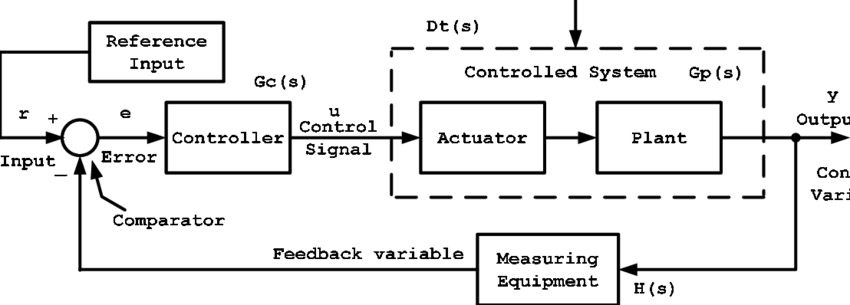
\includegraphics[scale=0.5]{closed-loop.png}
\end{center}
\begin{itemize}
\item Terminology
\begin{itemize}
\item \textbf{Plant}  - system to be controlled, the "physics" of the problem (e.g. UAV)
\item \textbf{Sensor} - measures quantities
\item \textbf{Actuator} - controls the plant (e.g. motor)
\item \textbf{Controller} - processors sensor data to drive actuator
\item \textbf{Control law} - algorithm used by control processor to compute actuator signal (math)
\end{itemize}
\item Example: hot plate temperature
\begin{itemize}
\item Equation $T=T_\text{amb}+\alpha(P+D)$ is used for output, where $P$ is input power, $D$ is external disturbance, $\alpha$ is in $^\circ\text{F}/\text{W}$
\item Using algebra, manipulate to solve for $P$, given a $T_\text{desired}$ - $P=\frac{T_\text{des}-T_\text{amb}}{\alpha}$, assuming $D$ is 0 W.
\item Error is $e=T-T_\text{des}$, goal is to have this be zero
\item In open loop control, have to manually adjust, with trial and error
\item Closed loop control equation:  $P=\frac{T_\text{des}-T_\text{amb}}{\alpha}-k(T-T_\text{des})$
\begin{itemize}
\item Increase power if too cold, lower power if too warm
\item Feed the error back into the system
\item The $k$ term can be optimized with trial and error
\end{itemize}
\item In the end,
\begin{equation*}
\text{closed-loop error}=\frac{\text{open-loop error}}{1+\alpha k}
\end{equation*}
\item Error is significantly less in closed-loop control when getting to a steady state
\end{itemize}
\item Slide camera example
\begin{itemize}
\item A camera moves along a fixed track with velocity $\vec{v}$ and camera pitch angle $\theta$, and its target position $x_\text{des}$ is at an angle $\gamma$ with respect to $\theta$
\item $\dot{x}=\vec{v} $ and $\dot{\vec{v}}=K\sin\theta$ 
\item Can detect $\gamma=-(\tan^{-1}(\frac{x-x_\text{des}}{h})+\theta)$ based on sensors in the camera frame, where $x$ is the current 2D position of the drone along the ground and $h$ is its height
\item Letting $u=\theta$ (controller to plant value), goal is to find $\theta(t)$ to control the drone that makes $\gamma\rightarrow\gamma_\text{des}$
\begin{itemize}
\item $\gamma_\text{des}=0$ is the general goal
\end{itemize}
\item In a simplified version, $\theta=0$ is is effectively ignored, and goal is to drive $\dot x=\vec{v}$ and find $\vec{v}(t)$
\begin{itemize}
\item  $\gamma=\tan^{-1}(\frac{x-x_\text{des}}{h})$, the angle between $x_\text{des}$ and $x$ with respect to the drone
\item Find an optimized $u=\vec{v}$  that drives $\gamma\rightarrow\gamma_\text{des}$ 
\item For a velocity command, $\vec{v}=K_p\gamma_\text{err}$
\item For an acceleration command, $\vec{a}=K_p\cdot\frac{d}{dt}\gamma_\text{err}(t)$
\item Integration of $\gamma_\text{err}(t)$ can be used to fix induced noise when sending velocity commands (e.g. due to wind)
\end{itemize}
\end{itemize}
\end{itemize}

\section*{PID Control}

\begin{equation*}
u(t)=\underbrace{K_P\cdot e(t)}_\text{current} + \underbrace{K_D \frac{d}{dt}e (t)}_\text{future}+\underbrace{K_I \int_0^t e(t)}_\text{past}
\end{equation*}
\begin{itemize}
\item Choosing gains
\begin{enumerate}
\item Increase $K_P$ until system starts to oscillate around the target, with other gains at $0$
\item Increase $K_D$ to damp motion/oscillation
\item Increase $K_I$ to get rid of steady state error
\end{enumerate}
\item $P$ is almost universal in all controllers
\begin{itemize}
\item May cause overshoot and oscillation, however
\end{itemize}
\item $I$ resolves steady-state error
\begin{itemize}
\item Risks causing saturation
\end{itemize}
\end{itemize}
\begin{itemize}
\item $D$ predicts future to avoid overshoot
\begin{itemize}
\item Noise can exaggerate derivative commands
\end{itemize}
\end{itemize}

\section*{Optical Flow}

\begin{itemize}
\item Motion field - 2D projection of 3D motion
\item Optical flow field - 2D, apparent motion; requires reflection
\item Despite 6 degrees of freedom, can  only capture a 2D field
\item Example: matte sphere rotating has motion field, but not an optical flow field
\item Process of visualization
\begin{itemize}
\item Two frames are given as input
\item Differences are computed and visualized
\end{itemize}
\item Applications
\begin{itemize}
\item Video stabilization
\item Denoising
\item Super resolution
\end{itemize}
\item Scanning locally (small window) for changes is more effective
\item Goal is to find differences between  two frames
\item Need to find corners and determine if they are same
\begin{itemize}
\item "Flat"region- no change in all directions
\item "Edge" - no change along edge direction
\item "Corner" - change in all directions (in uniform color shape)
\item Differences due to aliasing in images
\end{itemize}
\item Windows - spacial and temporal
\begin{itemize}
\item $u$ is translation in $x$ direction, $v$ is "wiggle" in $y$ 
\item Not moving window around, but see how contents will change over time
\end{itemize}
\end{itemize}
\begin{equation*}
E(u,v)=\sum_{x,y}\underbrace{w(x,y)}_\text{window function}[\underbrace{I(x+u,y+v)}_\text{shifted intensity}-\underbrace{I(x,y)}_\text{intensity}]^2
\end{equation*}
\begin{itemize}
\item Change in appearance for the shift, as a function of pixel intensities
\item Trial and error required to determine appropriate $u$ and $v$ 
\item Window function is a weighted sum of the pixels in the window
\item $u$ and $v$ are $(0, 0)$ if the image is the same color throughout
\item Small but nonzero shifts in $u$ and $v$ are interesting to find out, key to edge detection
\item Taylor series - approximation of a function by taking the derivative throughout its input
\item Product rule: $\frac{d}{dx}f(x)g(x)=f'(x)g(x)+f(x)g'(x)$
\item For an image corner,
\end{itemize}
\begin{equation*}
M=\begin{bmatrix}
\sum I_x^2&\sum I_xI_y\\\sum I_xI_y&\sum I_y^2
\end{bmatrix}\approx 
\begin{bmatrix}
\lambda_1&0\\0&\lambda_2
\end{bmatrix}
\end{equation*}

\begin{itemize}
\item Eigenvalues help define shape of an ellipse, in terms of stretch/compression factors
\begin{itemize}
\item $\lambda_1$ is the direction of the fastest change, independent of $\lambda_2$ 
\end{itemize}
\item Harris Detector Algorithm
\begin{itemize}
\item Has translation and rotation invariance
\item No scalar invariance - zooming in on a corner reveals multiple "edges"
\item Detects glare and lighting changes easily, yet still identify object
\end{itemize}
\item "Phase diagram" based on actual phase gives probablistic, fast realtime estimation of object
\item Optical flow has many methods
\begin{itemize}
\item Pixel difference for every pixel
\item Corner detection
\end{itemize}
\item Only is apparent motion of object
\begin{itemize}
\item Problem occurs when motion vectors of individual pixels are in different directions
\item The pixel correspondence problem - how to estimate pixel motion
\end{itemize}
\item Assumptions made in computing optical flow
\begin{itemize}
\item Brightness/intensity of pixel is constant between frames (brightness constancy)
\begin{itemize}
\item Problem when lighting changes
\item $I(x,y,t)=I(x+u,y+v,t+1)$, once we know $u$ and $v$ 
\end{itemize}
\item Solving equation with Taylor series,  we get $I(x+u,y+v)=I(x,y,t+1)+\frac{\partial I(t)}{\partial x}u+\frac{\partial I(t)}{\partial y}v$, but only applicable for small motions
\item Derivation from smoothness is Gaussian
\end{itemize}
\item Aperture problem - if the window is too small, apparent motion direction may not be the actual direction
\begin{itemize}
\item Solution is to pretend adjacent pixels have the same $(u,v)$ in a window with $n$ pixels

\begin{equation*}
\begin{bmatrix}
I_x(p_1)&I_y(p_1)\\\vdots&\vdots\\I_x(p_n)&I_y(p_n)
\end{bmatrix}
\begin{bmatrix}
u\\v
\end{bmatrix}=
\begin{bmatrix}
I_{t_x}(p_1)&I_{t_y}(p_1)\\\vdots&\vdots\\I_{t_x}(p_n)&I_{t_y}(p_n)
\end{bmatrix}
\end{equation*}
\end{itemize}
\item Spacial smoothness - detect a whole  surface in space, based on edges
\end{itemize}
\end{document}
 